\begin{figure}[h!]
    \centering
    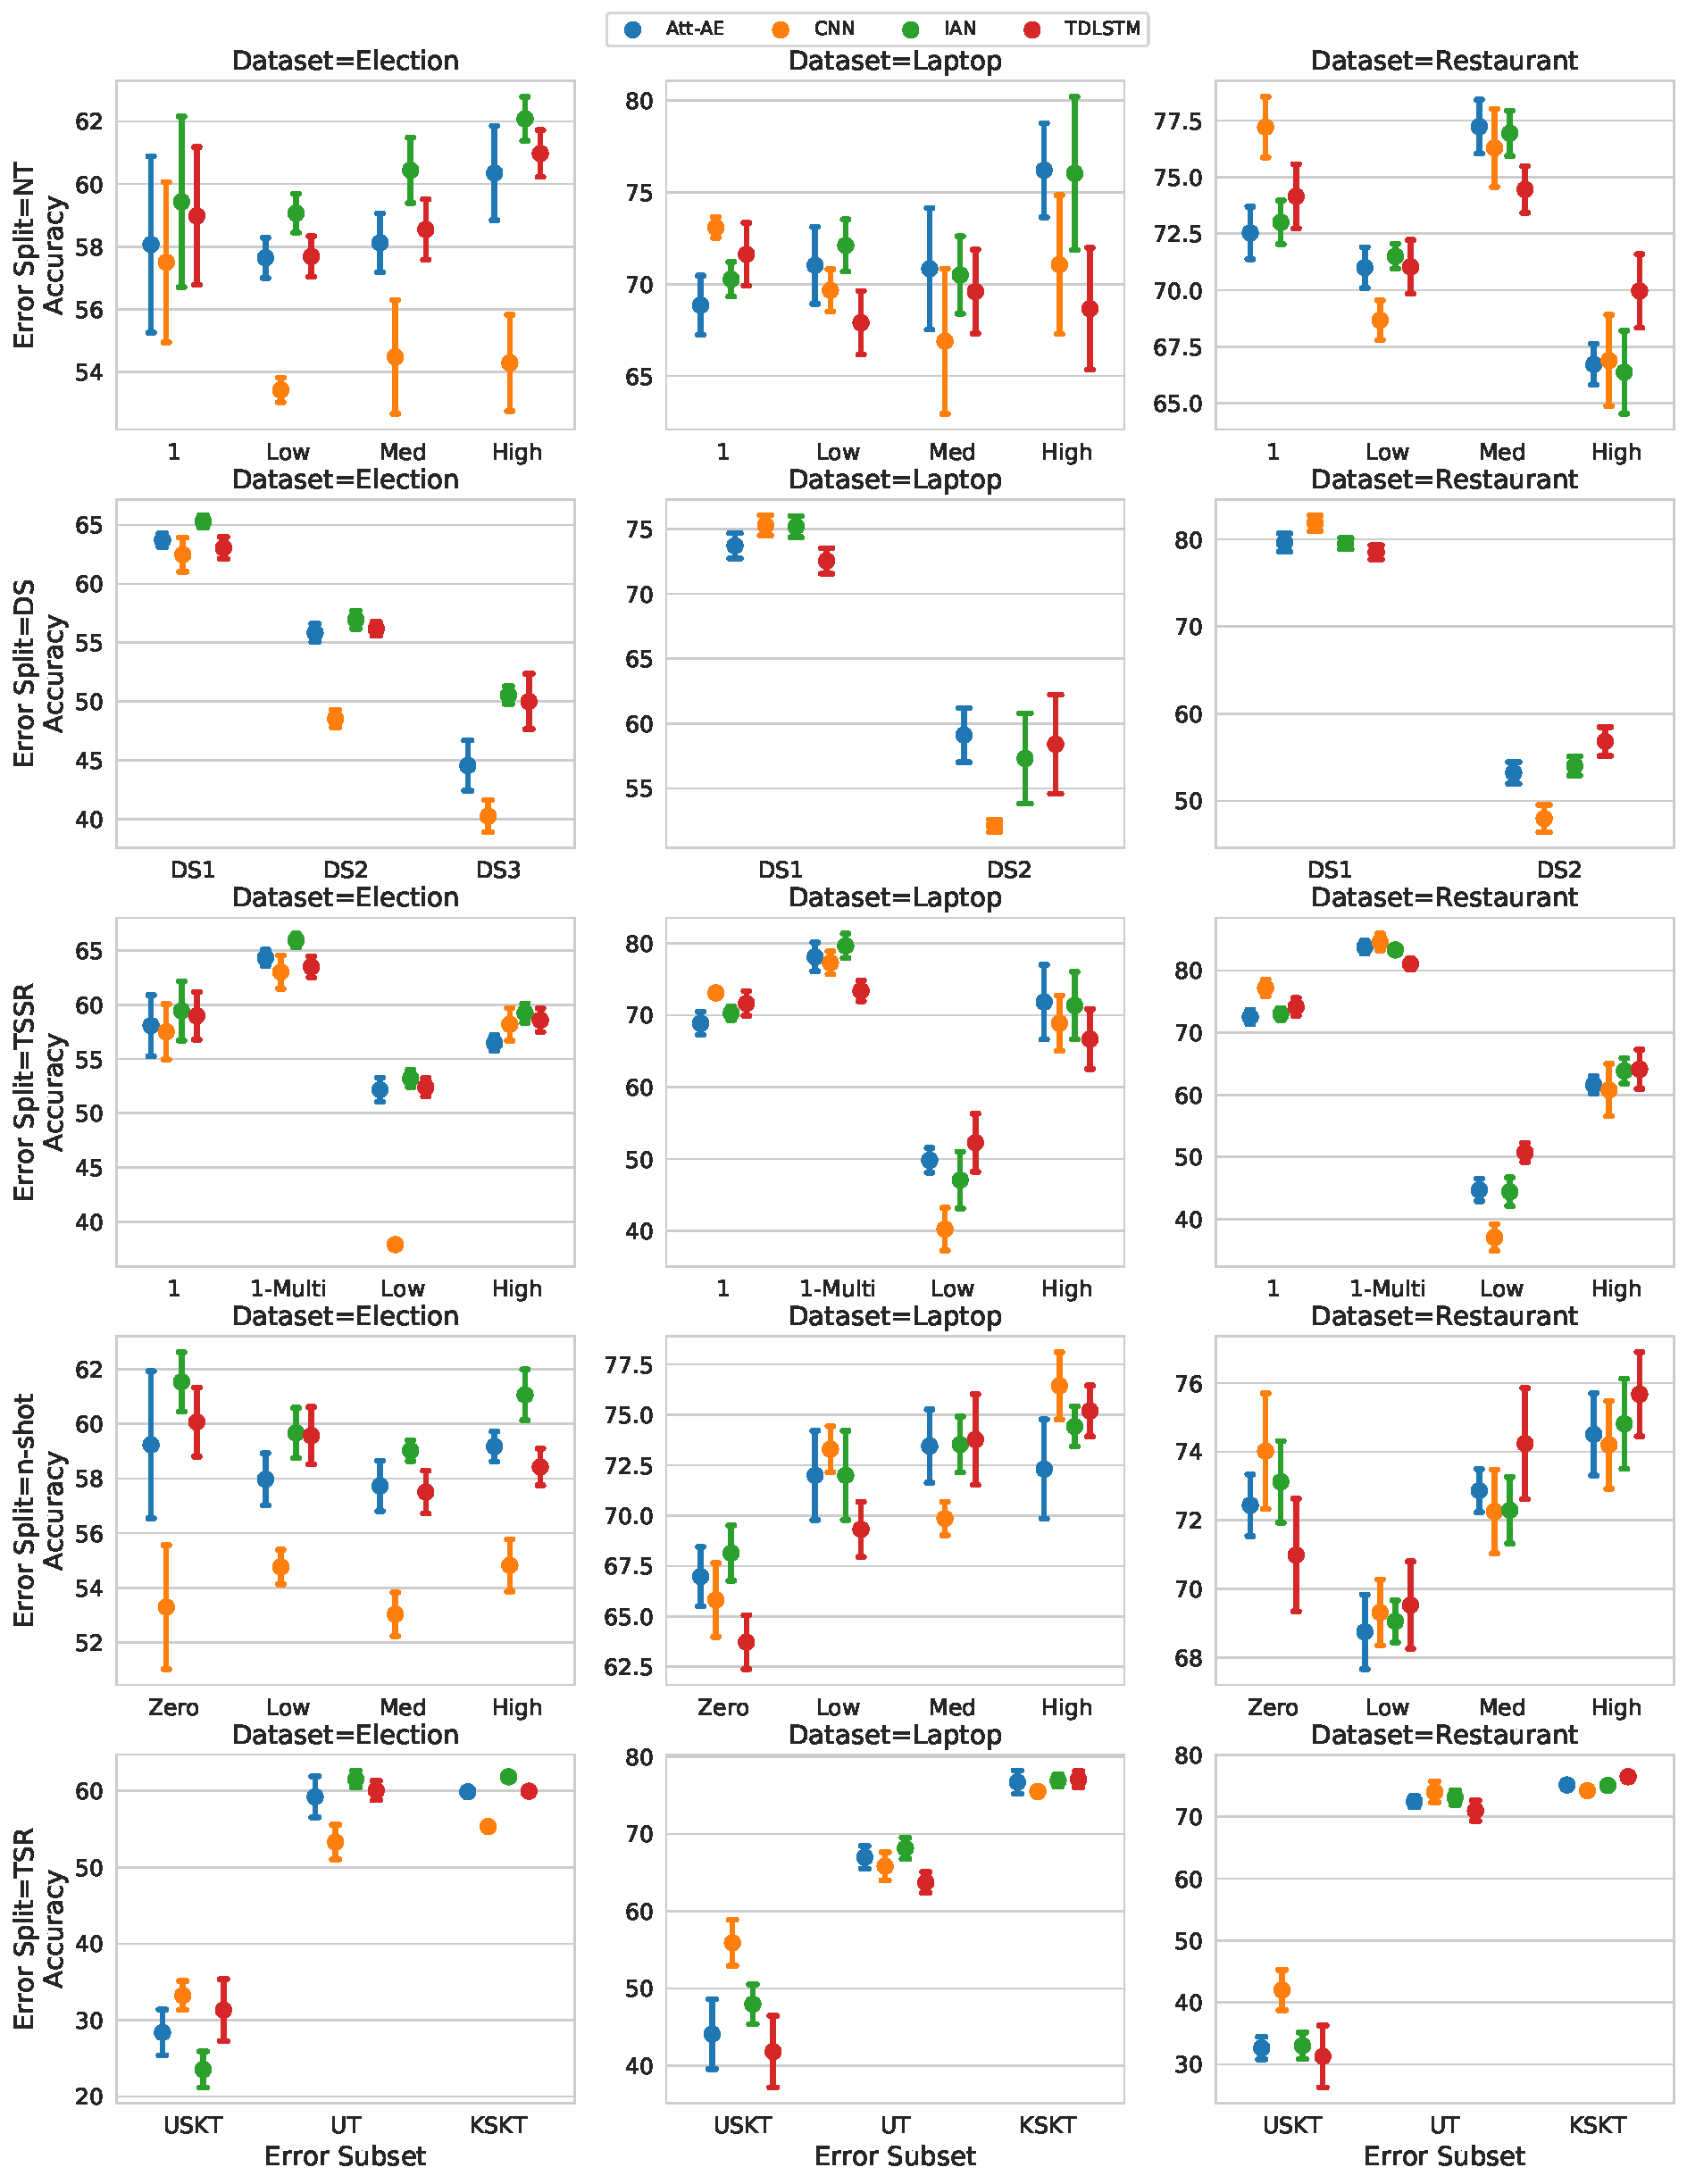
\includegraphics[scale=0.42]{images/augmentation/methods_performance/baseline/validation_error_subsets.pdf}
    \caption{The mean and standard deviation error bars for each error subset within all of the error splits on the validation split across all datasets.}
    \label{fig:aug_baseline_validation_error_subset}
\end{figure}

\begin{figure}[h!]
    \centering
    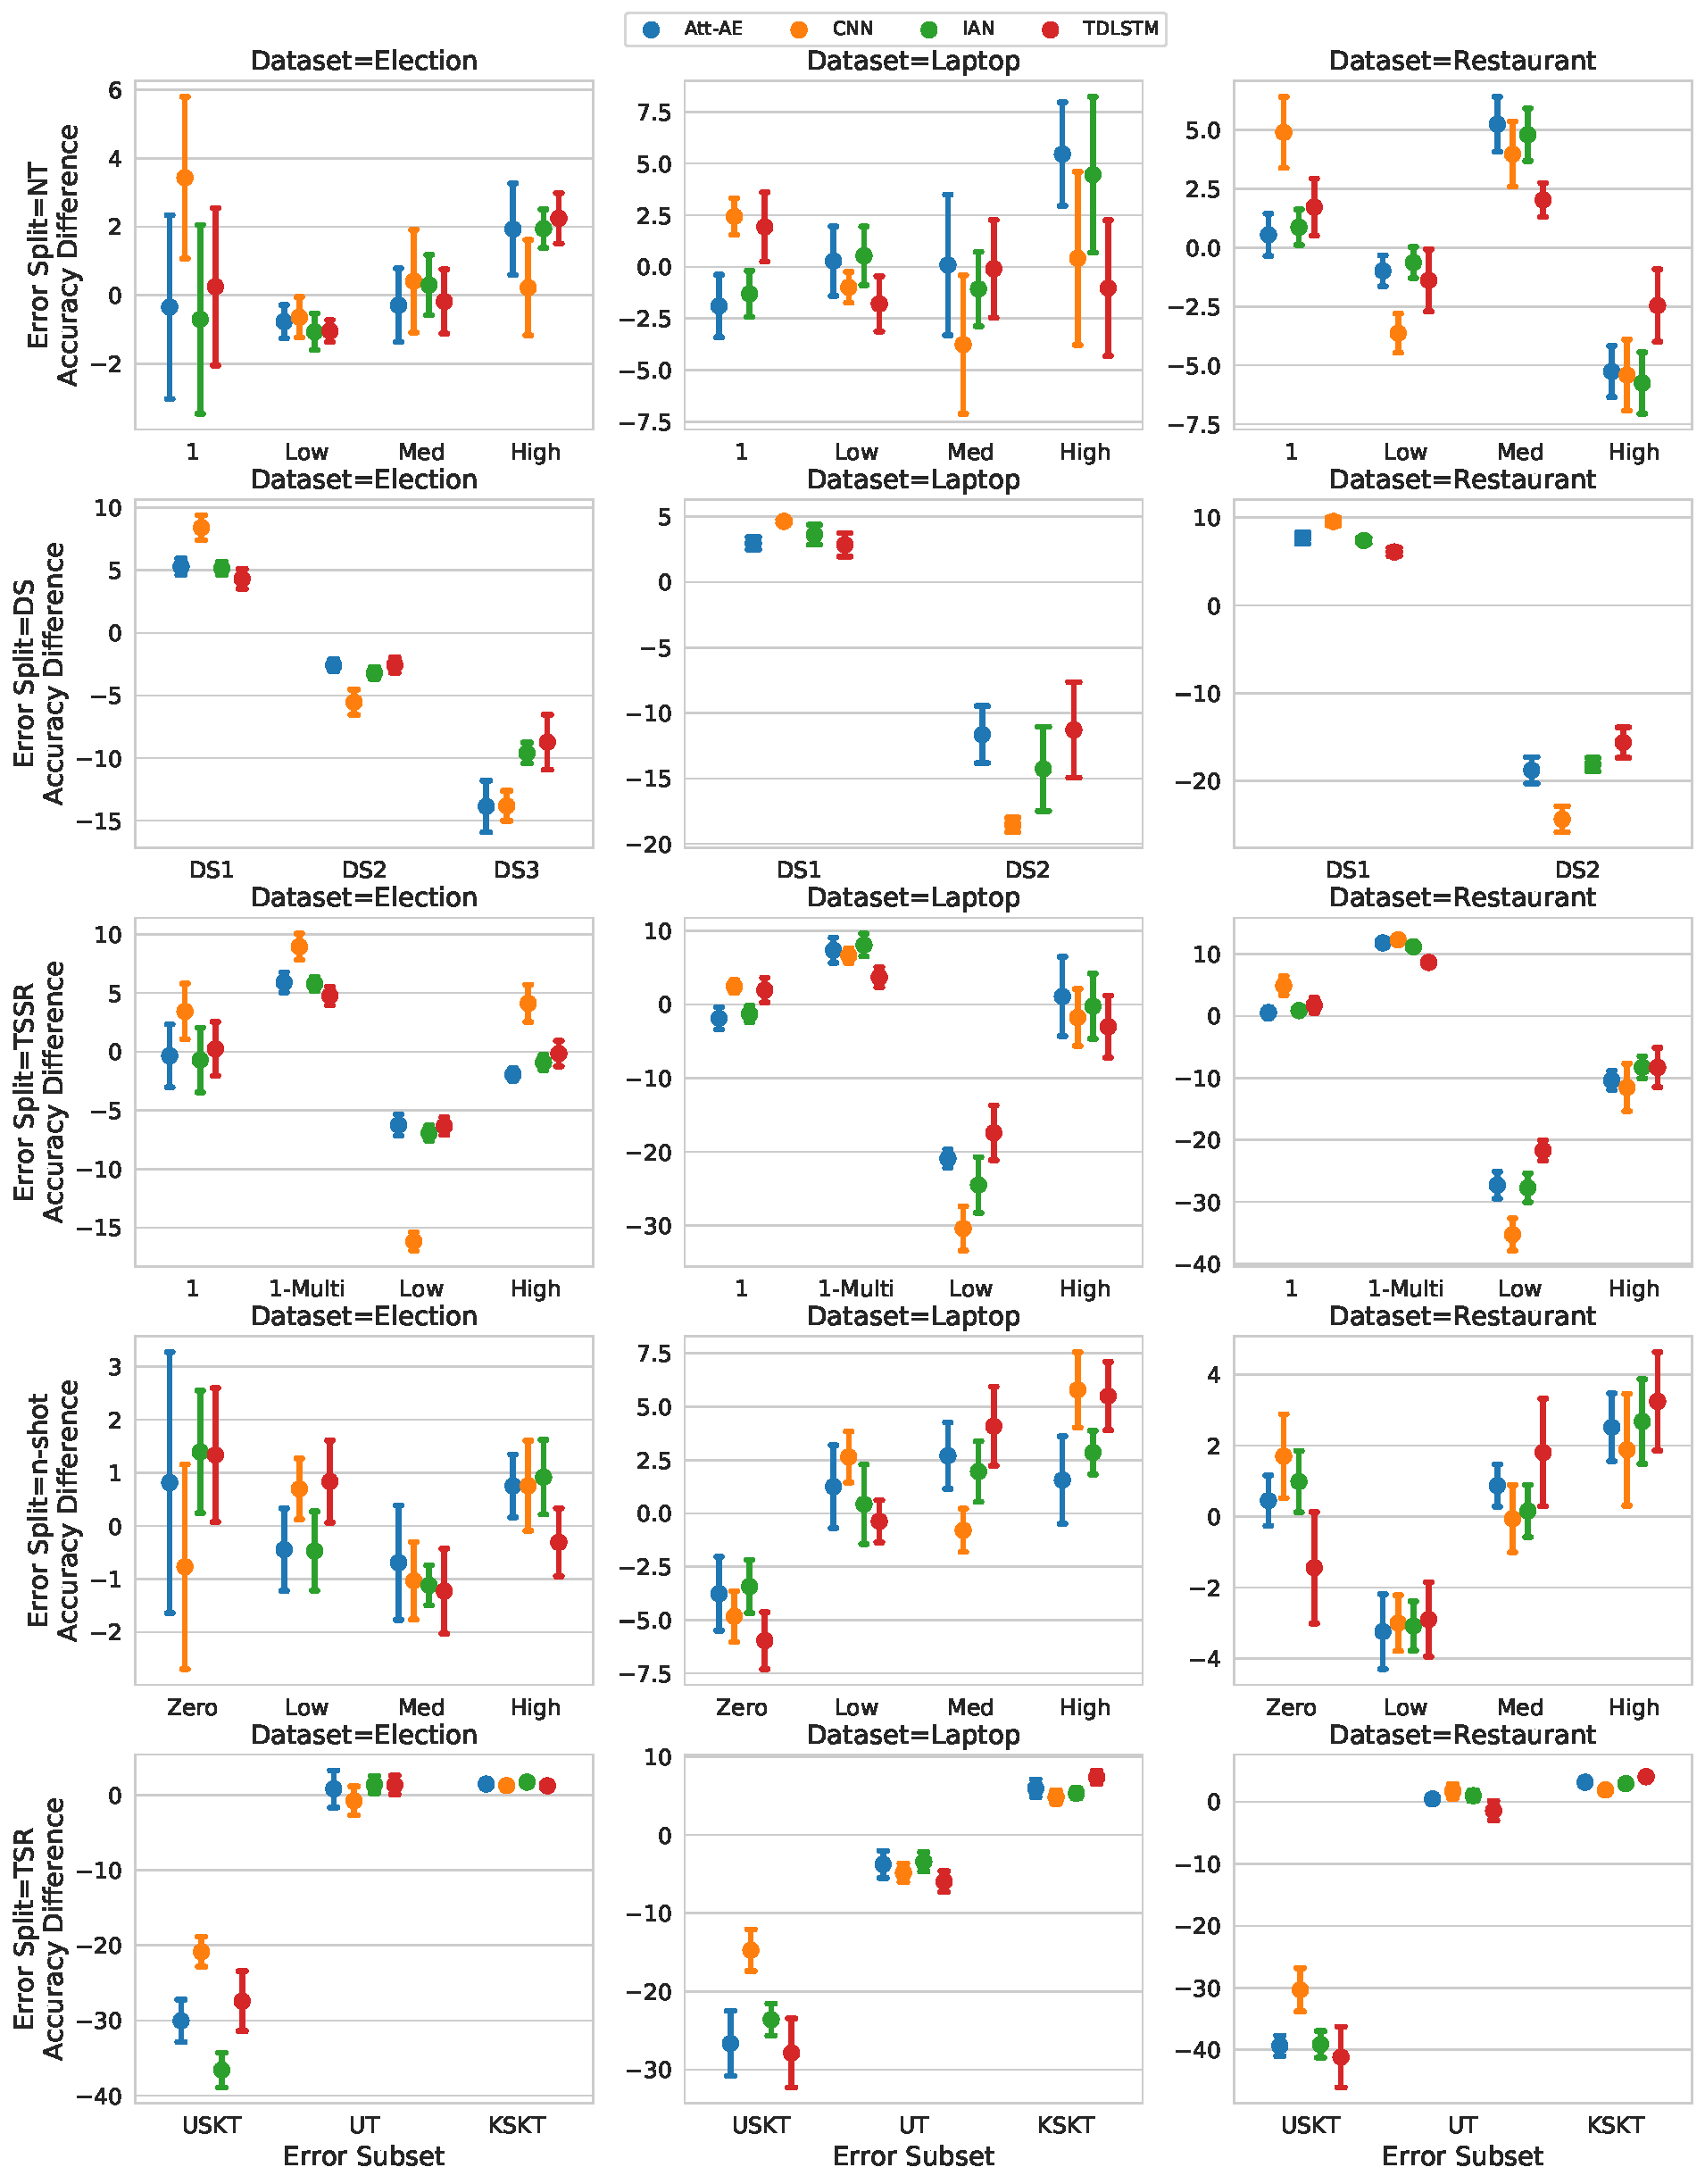
\includegraphics[scale=0.42]{images/augmentation/methods_performance/baseline/validation_error_diff_subsets.pdf}
    \caption{The mean and standard deviation error bars for the difference between the overall accuracy and the accuracy from each error subset within all of the error splits on the validation split across all datasets.}
    \label{fig:aug_baseline_validation_error_diff_subset}
\end{figure}

\begin{figure}[h!]
    \centering
    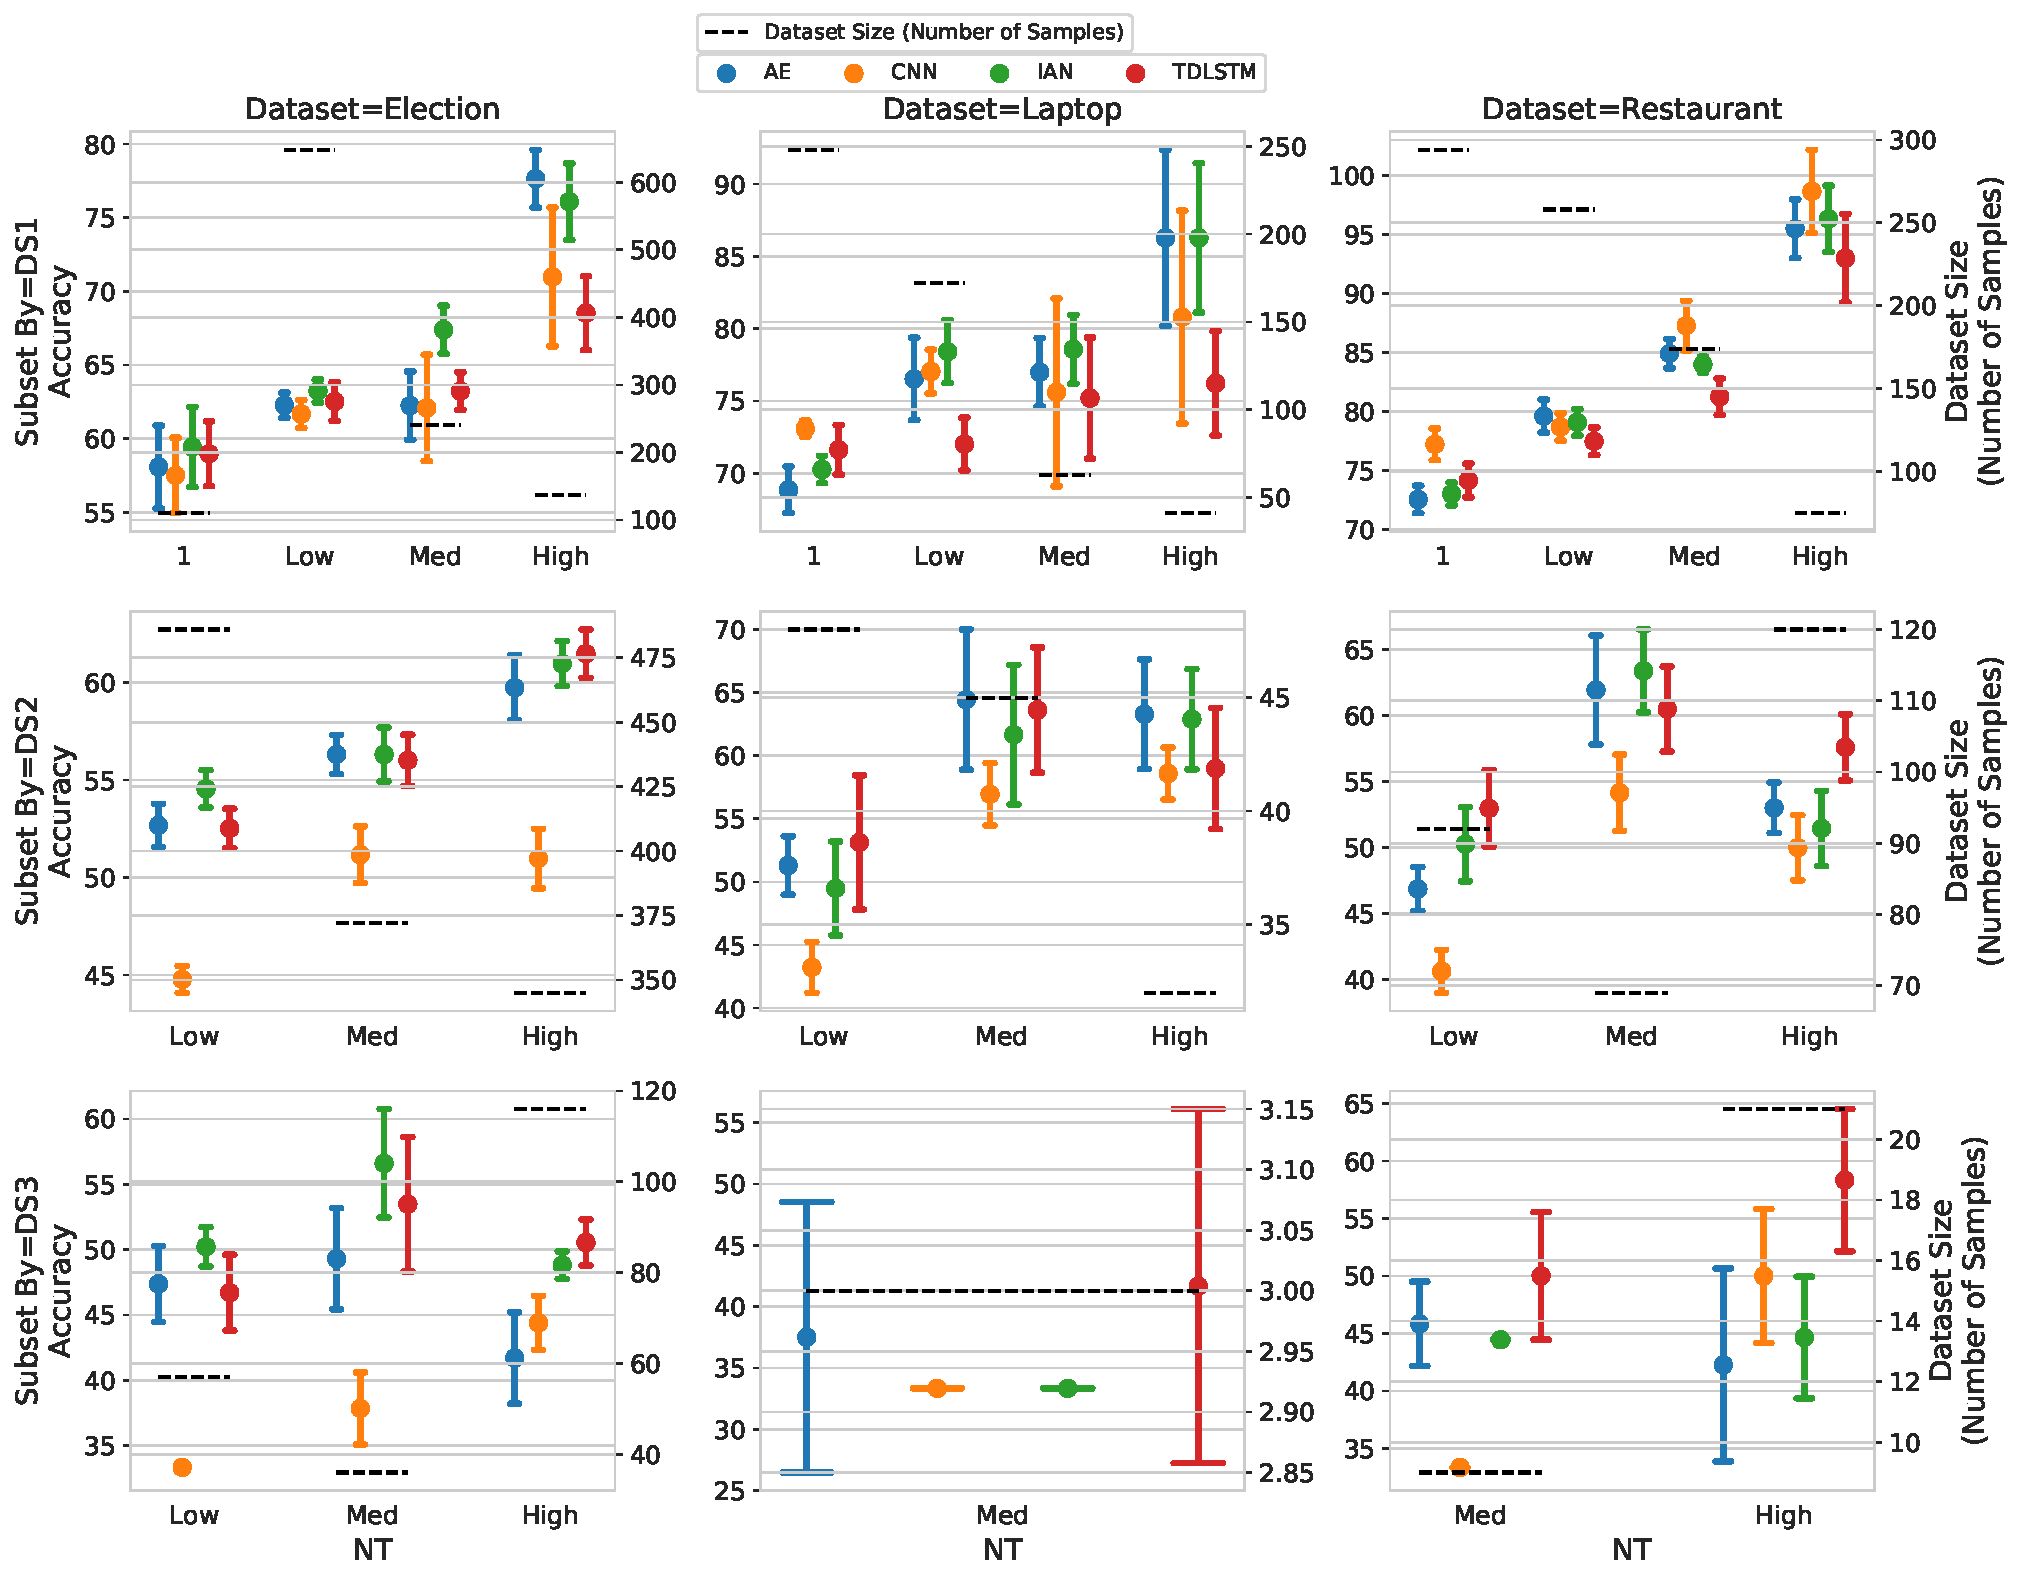
\includegraphics[scale=0.4]{images/augmentation/methods_performance/baseline/baseline_ds_nt_validation_scores.pdf}
    \caption{Each plot shows the performance (y-axis accuracy) of the given models and sample size of the data evaluated on (y-axis dataset size) on the different validation datasets (columns) after being subsetted by the relevant \textit{DS} subset (rows) and then NT subset (x-axis).}
    \label{fig:aug_baseline_ds_nt_validation_scores}
\end{figure}

\begin{figure}[h!]
    \centering
    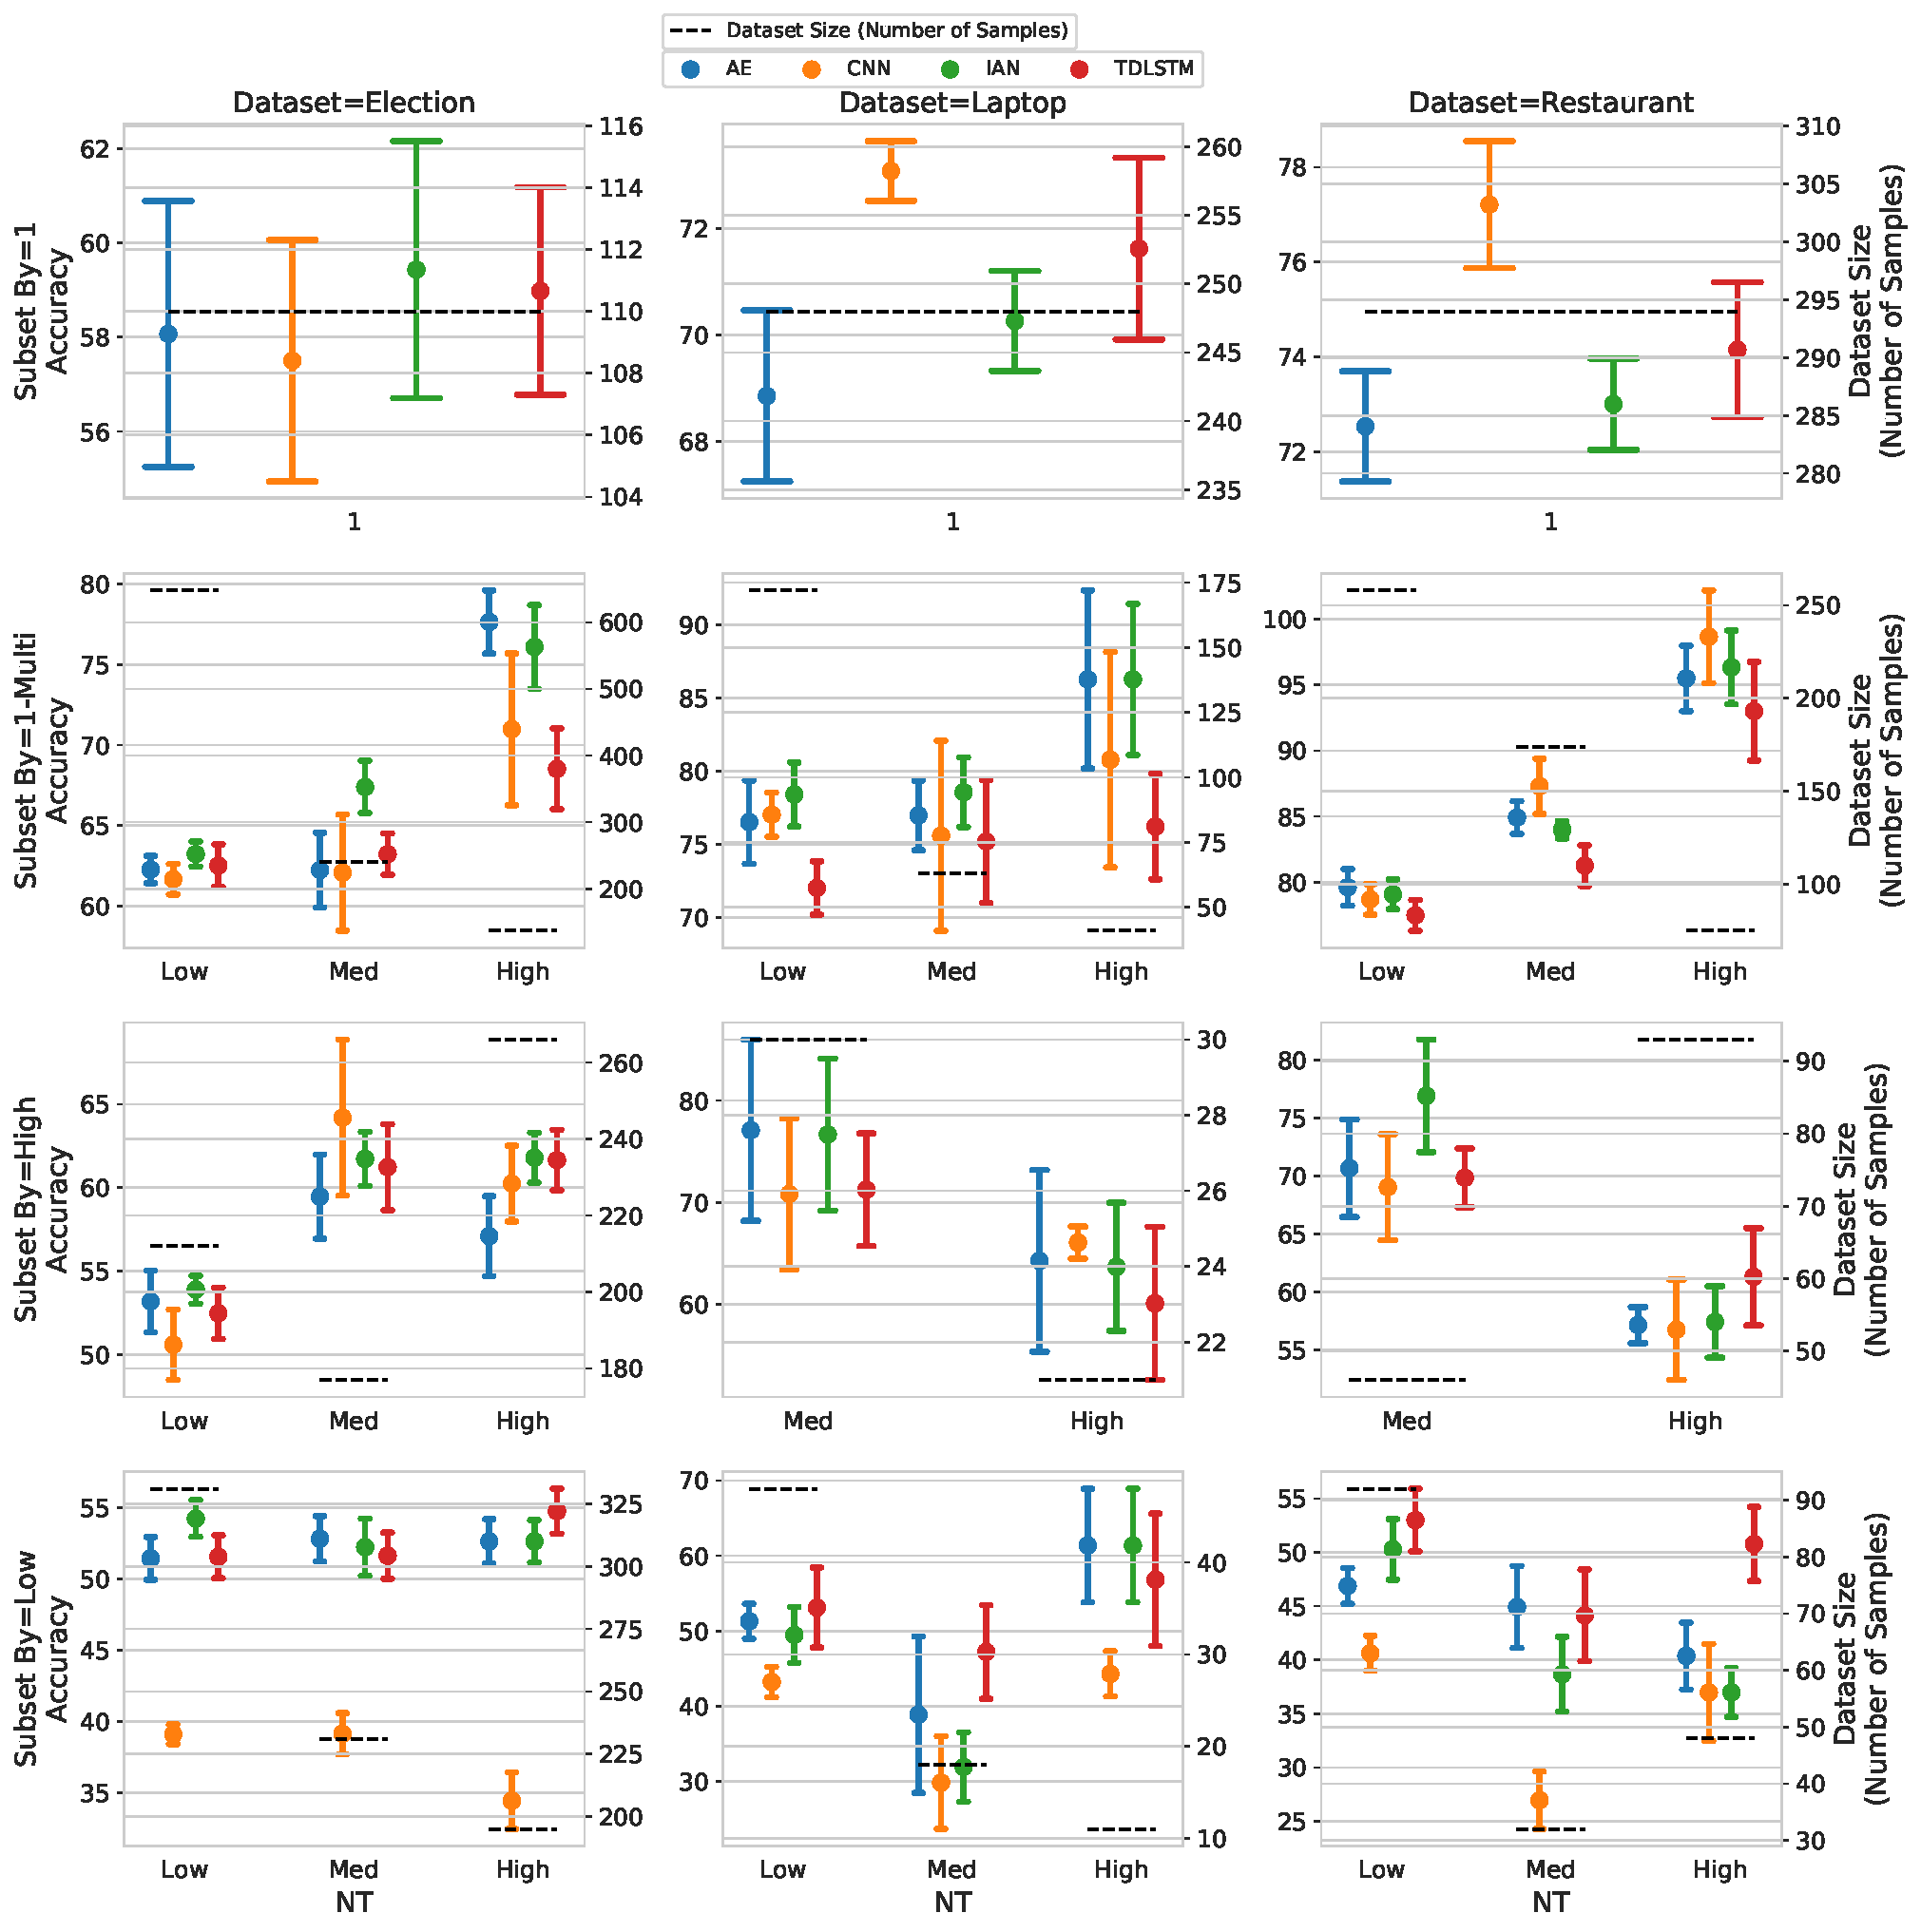
\includegraphics[scale=0.4]{images/augmentation/methods_performance/baseline/baseline_tssr_nt_validation_scores.pdf}
    \caption{Each plot shows the performance (y-axis accuracy) of the given models and sample size of the data evaluated on (y-axis dataset size) on the different validation datasets (columns) after being subsetted by the relevant \textit{TSSR} subset (rows) and then NT subset (x-axis).}
    \label{fig:aug_baseline_tssr_nt_validation_scores}
\end{figure}